\chapter{Architektur}
\section{Android Wear Paket Architektur}
Android Wear hat eine strikte Paket Architektur. Abbildung 7.1 veranschaulicht die Übersicht diese Architektur. Eine Android Wear App muss immer zwingend eine dazugehörige Android App beinhalten. Wenn beide Apps gemeinsam verwendete Klassen haben, müssen diese in ein solches Paket augelagert werden. Android Klassen können nicht in einer Android Wear Applikation instanziert werden. Üblicherweise wird bei der Installation der .apk auf ein Android Smartphone, parallel die Smartwatch App auf die Uhr mit installiert.
\begin{figure}[h]
  \centering
  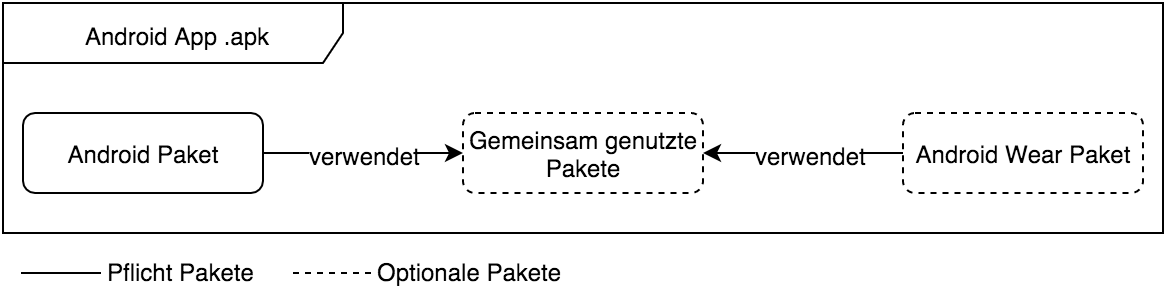
\includegraphics[scale=0.4]{98_Bilder/07_Architektur/AndroidPaketArchitektur}
  \caption[Übersicht Android Wear Paket Architektur]{Übersicht über die einzuhaltende Paketstruktur}
\end{figure}
\section{siot.net Applikationsarchitektur}
Die Architektur auf der Abbildung 7.2 definierte und ersichtliche muss eingehalten. Android und Android Wear Applikation für siot.net können so am effizientesten konzipiert werden.
\begin{figure}[h]
  \centering
  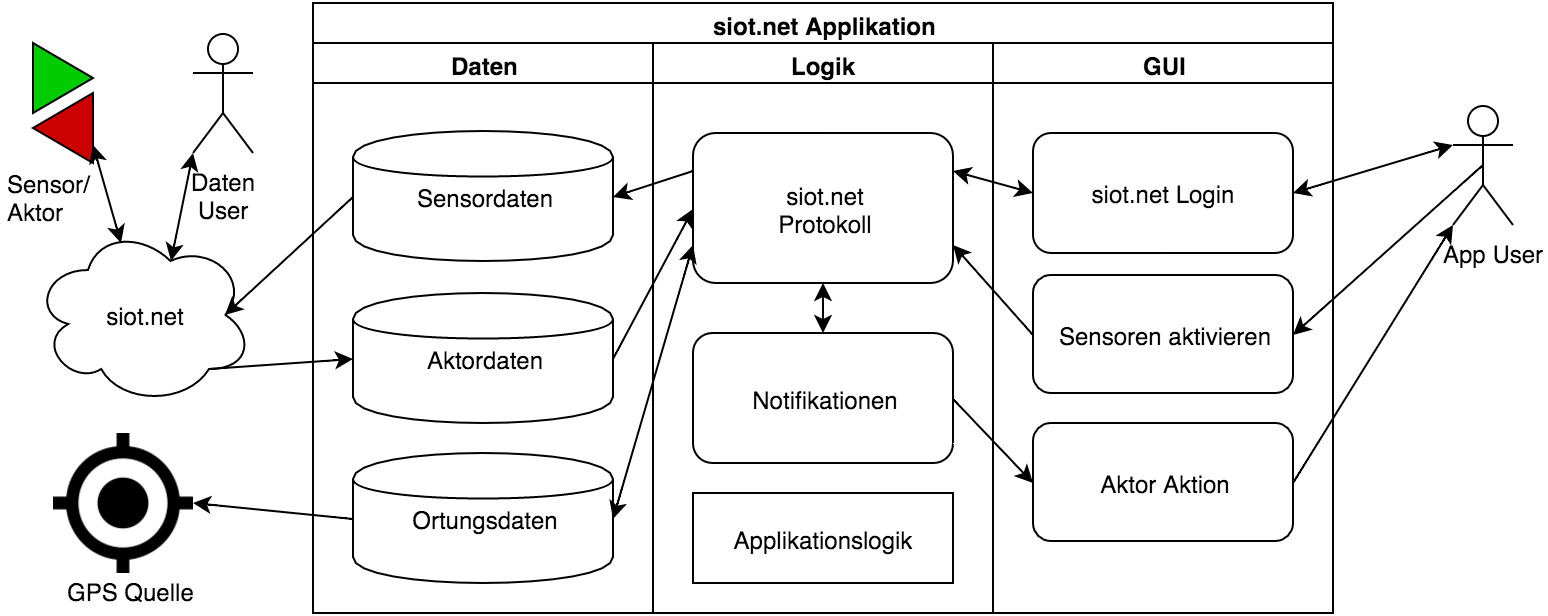
\includegraphics[scale=0.3]{98_Bilder/07_Architektur/siotAppArchitektur}
  \caption[Übersicht siot.net Applikationsarchitektur]{Applikationsarchitektur für siot.net Anwendungen}
\end{figure}
\section{Netzwerk-Architektur}
\subsection{geplante Architektur}
\begin{figure}[h]
  \centering
  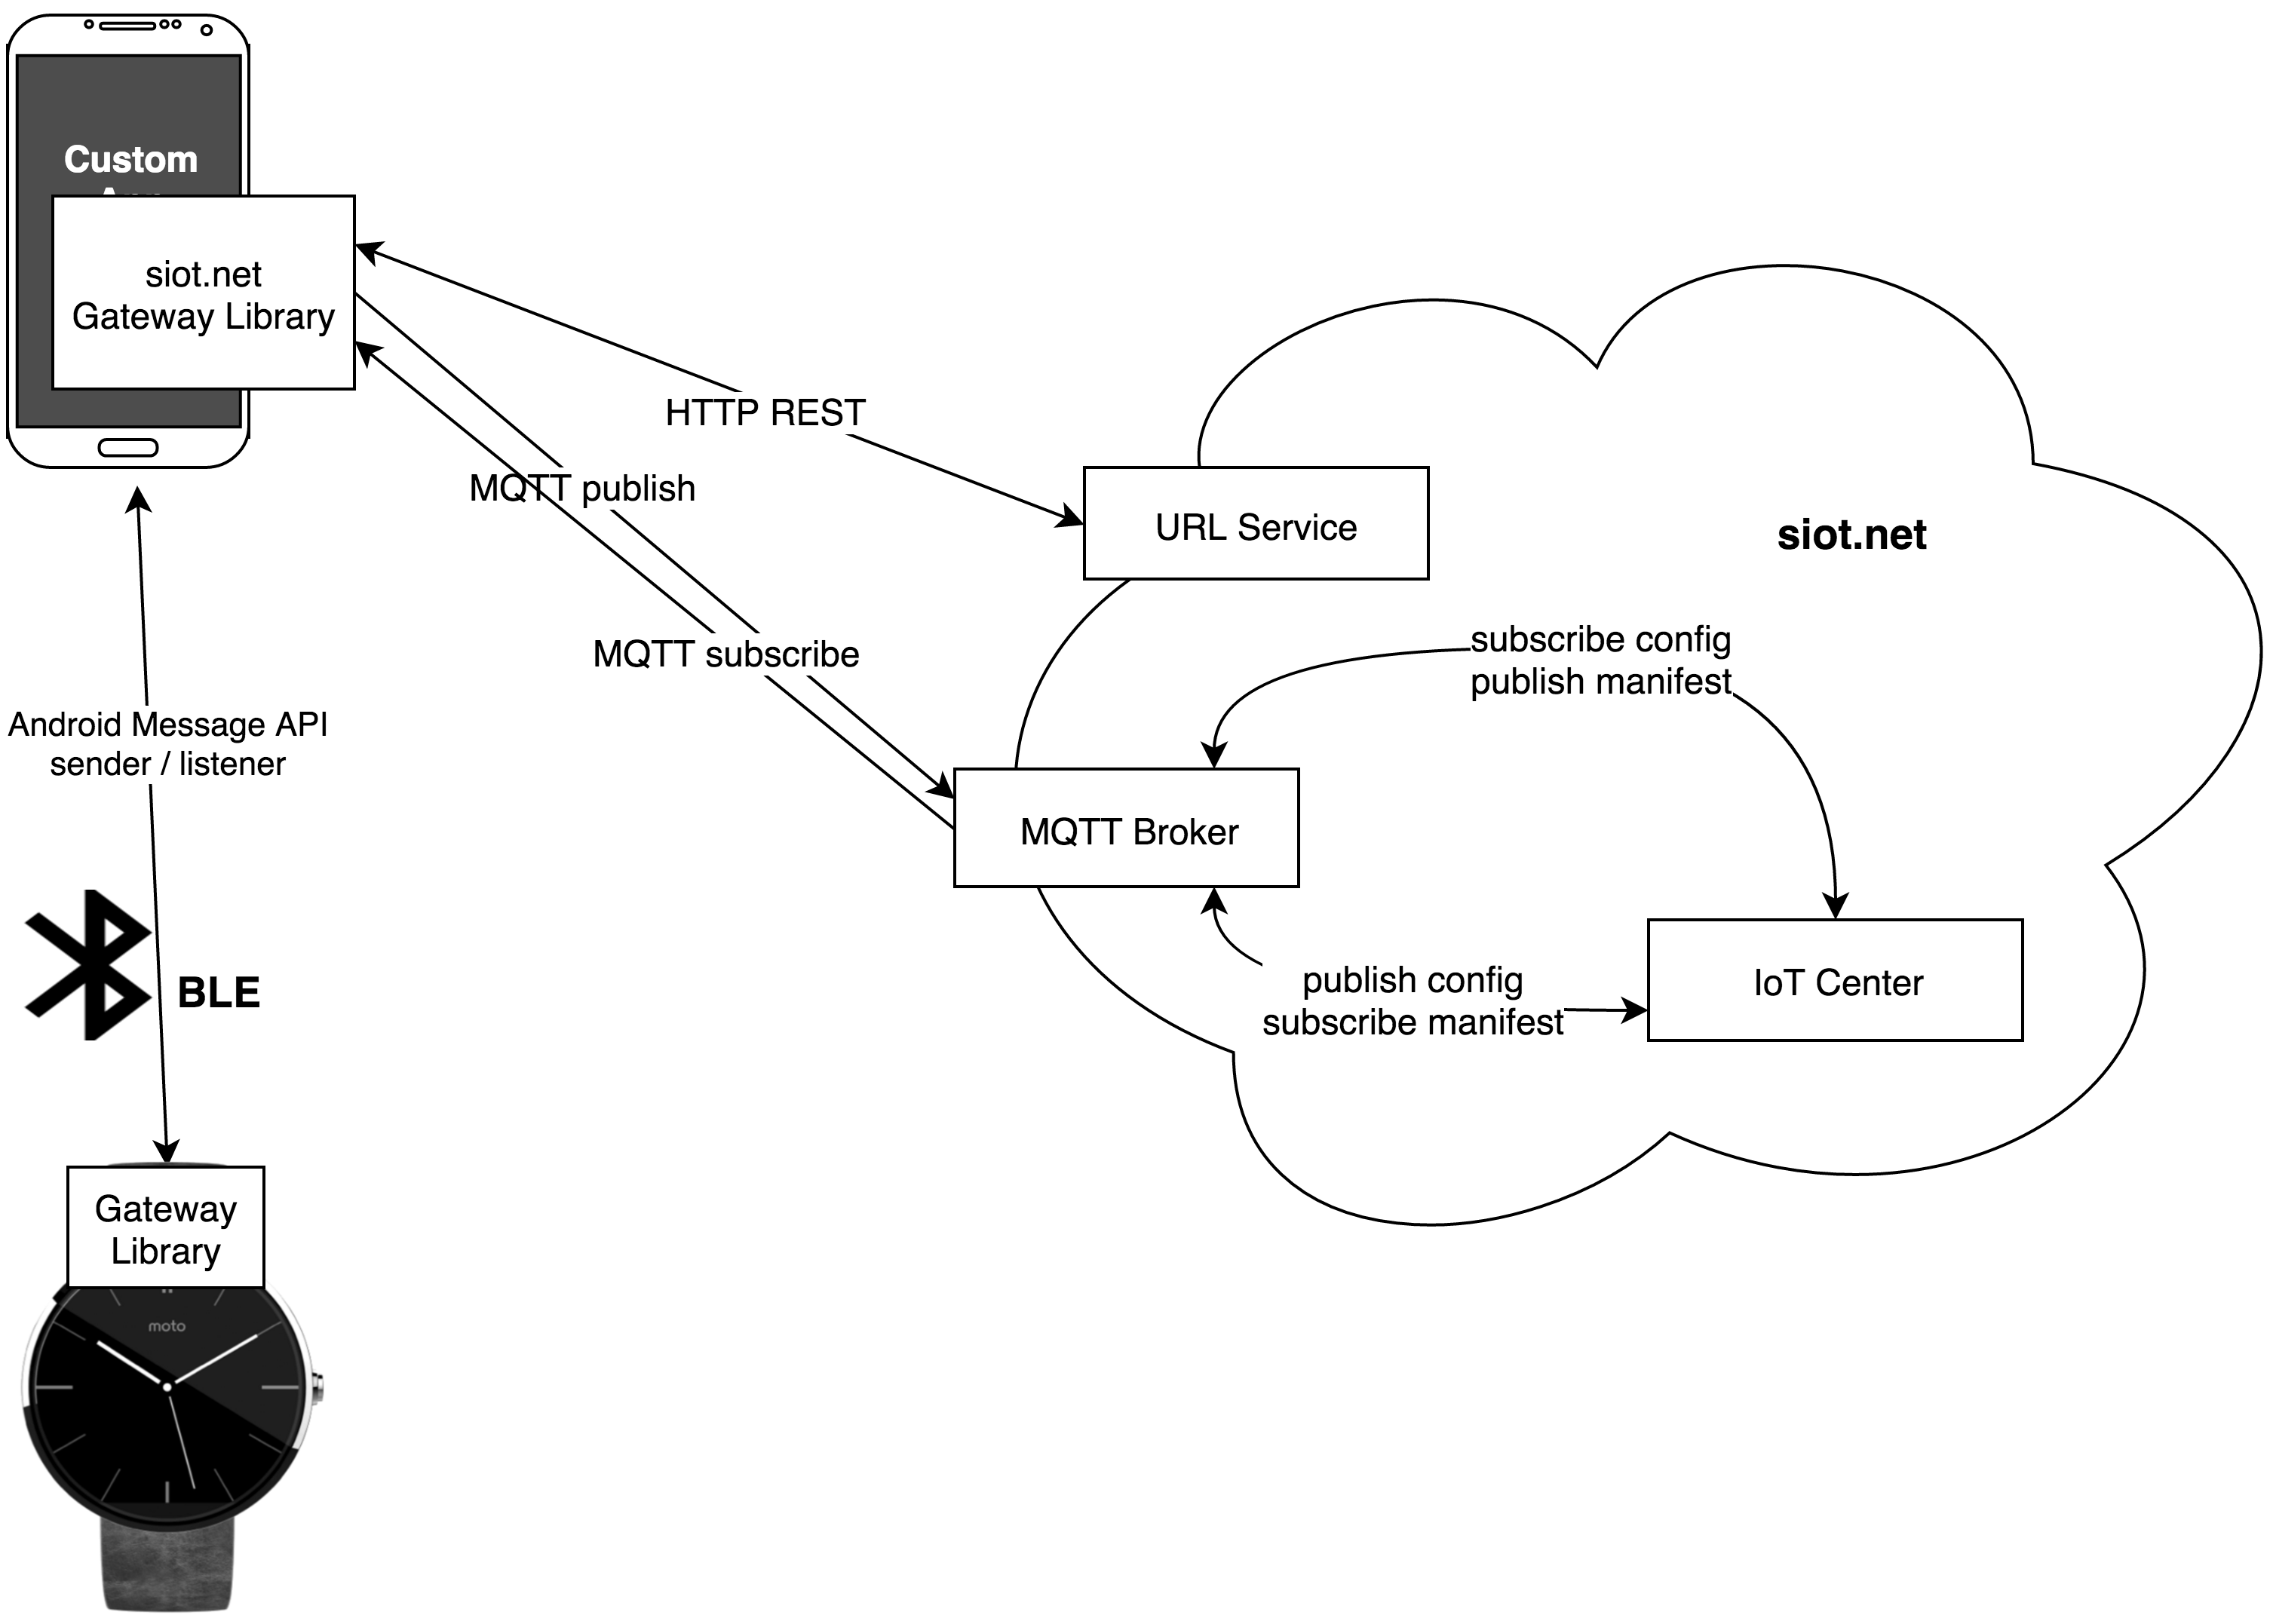
\includegraphics[scale=0.15]{98_Bilder/07_Architektur/01_Architektur}
  \caption[Geplante Netzwerk-Architektur mit BLE/ohne WLAN]{Geplante Kommunikation zwischen Smartwatch und Smartphone, sowie Smartphone und siot.net}
\end{figure}
In der Abbildung 7.3 visualisiert, wie die Kommunikation zwischen der Smartwatch, dem Smartphone und der siot.net Plattform stattfinden soll. Im Falle, dass die Smartwatch eine Bluetooth Low Energy (BLE) Verbindung mit dem Smartphone aufweist, wird dieses via REST und MQTT, mit siot.net Daten austauschen. Dabei dient das Mobiltelefon als Datenbrücke von der Smartwatch zur IoT-Cloud. Die Android Wear Uhr versendet die Daten, per Android Message API via BLE, zum Android Smartphone, das leitet die Pakete mit Hilfe des MQTT Protokoll weiter ans siot.net. Diese Variante der Datenübermittlung ist sehr viel stromsparender als die in Abbildung 7.4 gezeigte.\\
Das Bridging muss in der Smartphone Begleitapp (Android Paket) der Smartwatch Applikation (Android Wear Paket) implementiert sein.
\newpage
\begin{figure}[h]
  \centering
  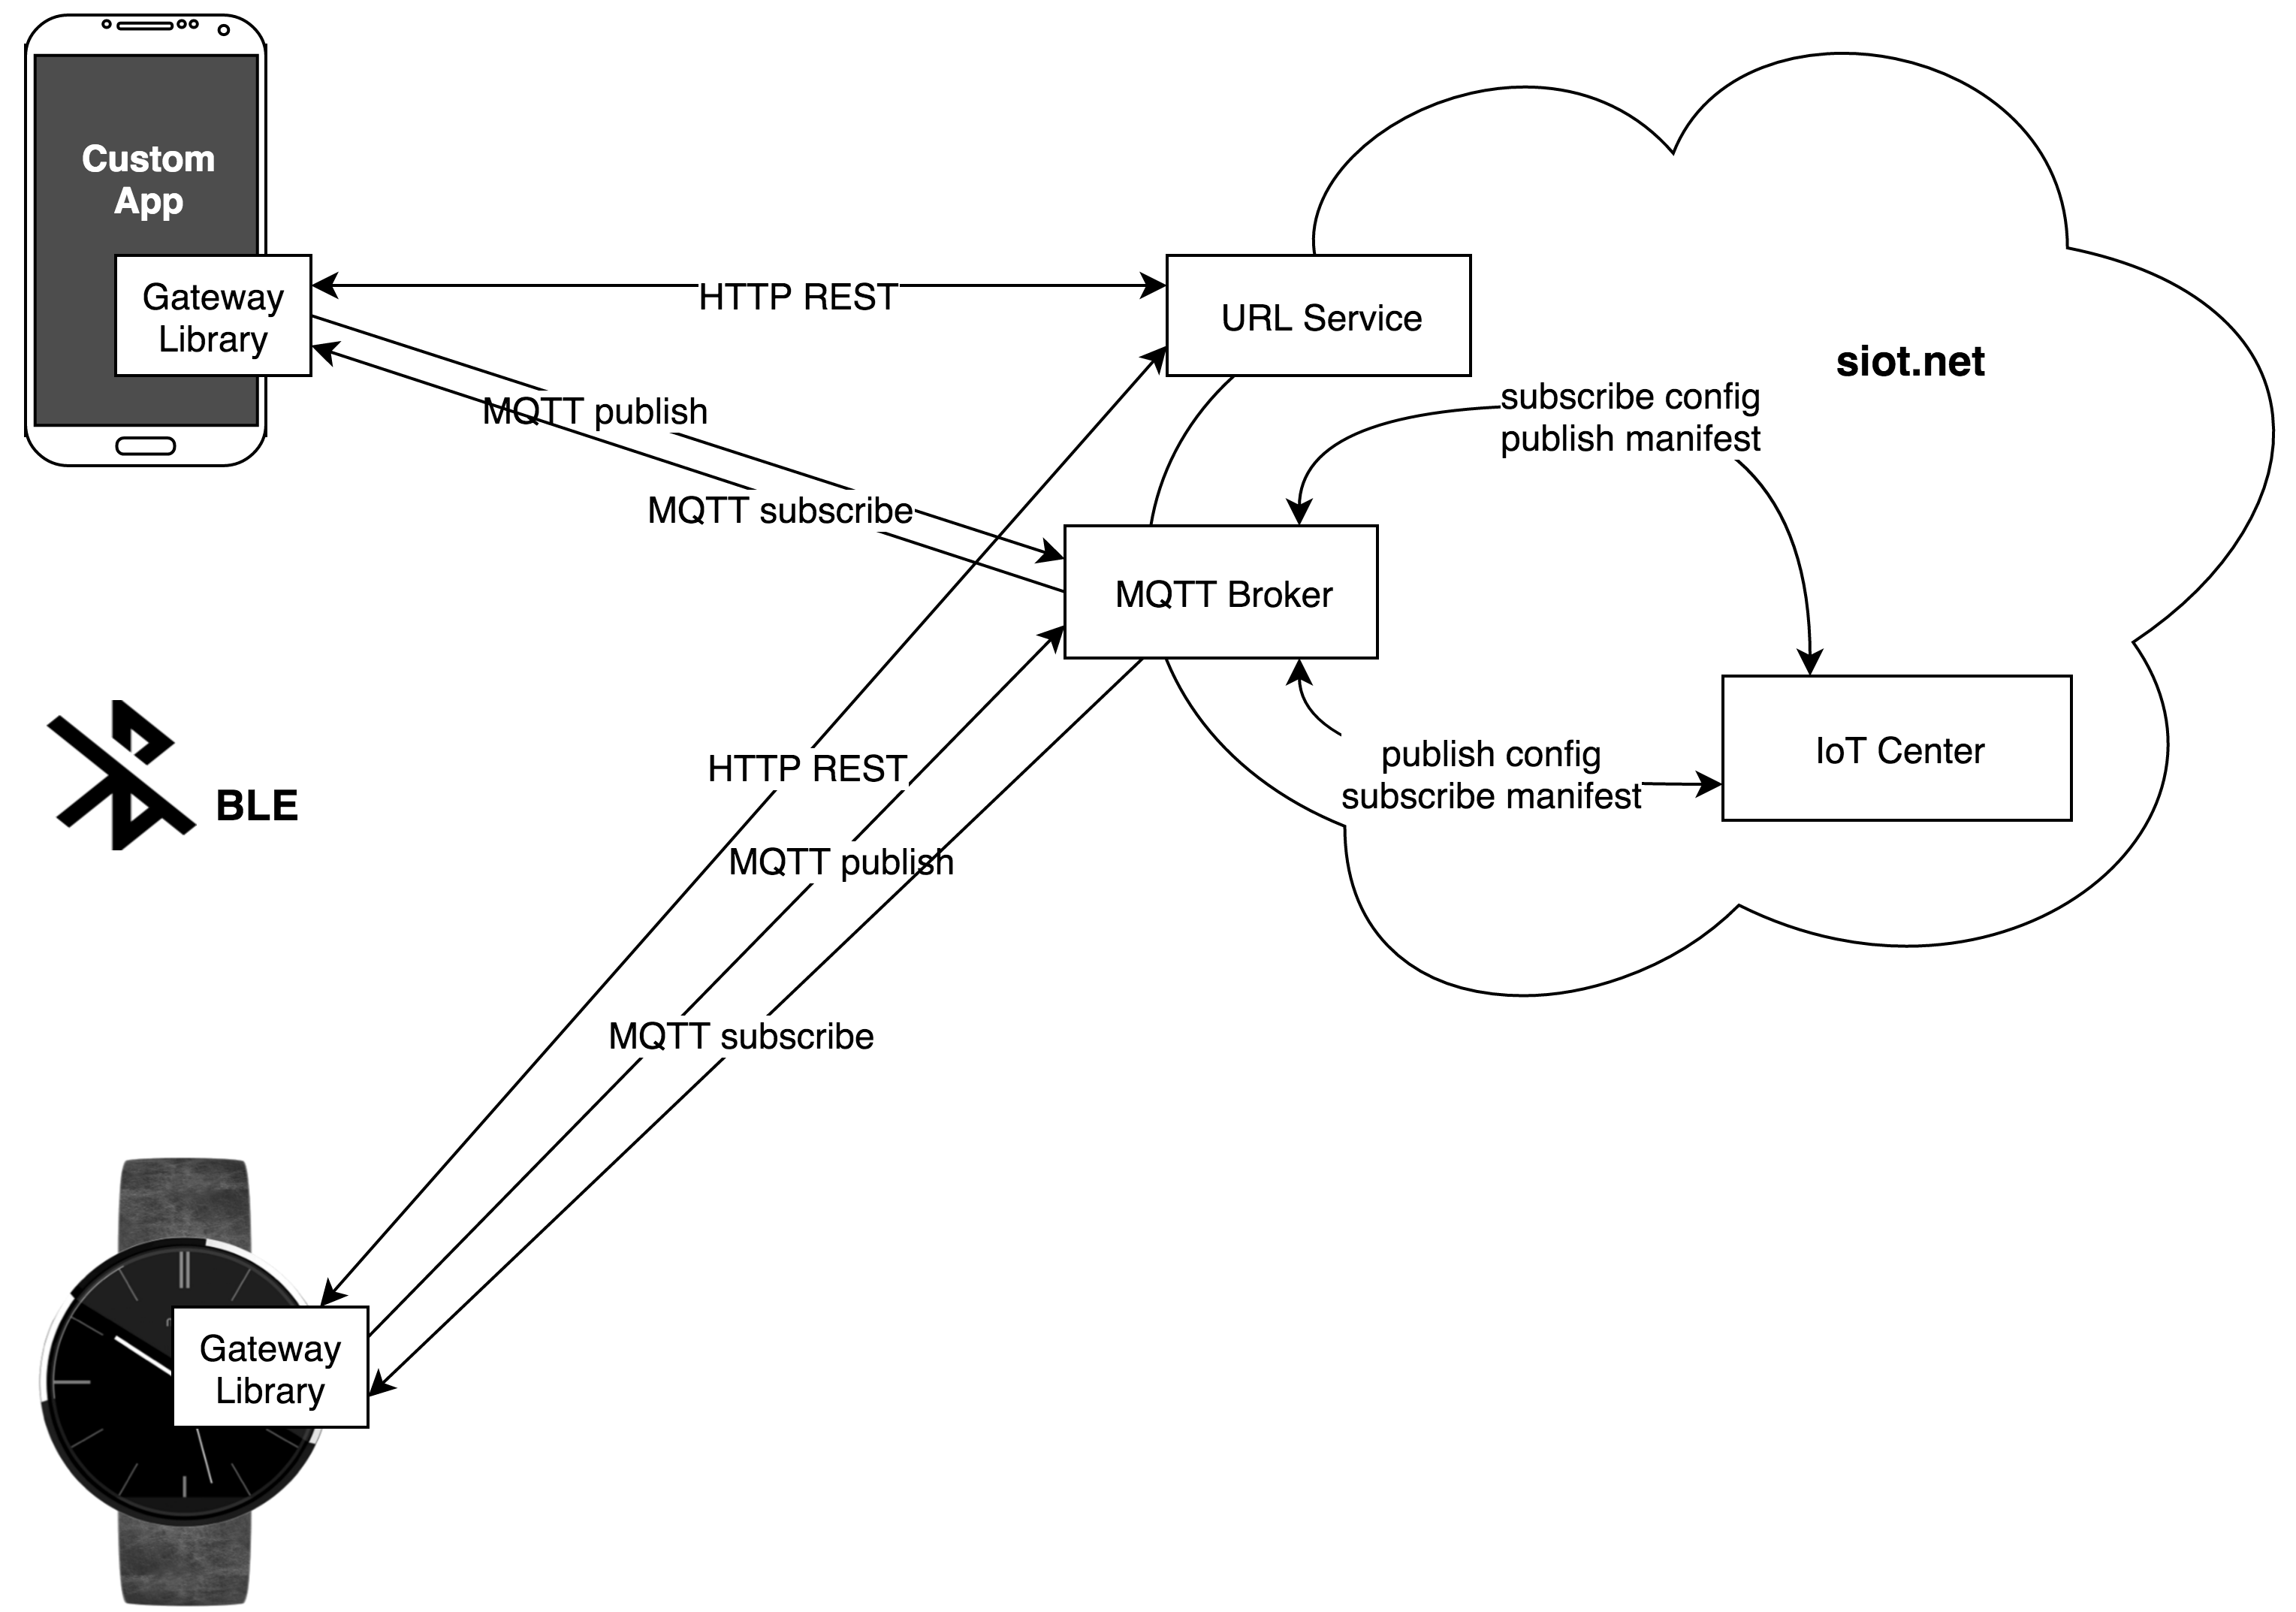
\includegraphics[scale=0.15]{98_Bilder/07_Architektur/02_Architektur}
  \caption[Geplante Netzwerk-Architektur ohne BLE/mit WLAN]{Geplante Kommunikation zwischen Smartwatch und siot.net, sowie Smartphone und siot.net}
\end{figure}
Bei Abbruch der Verbindung von Smartwatch zu Smartphone, soll die Computeruhr die Kommunikation zum siot.net selber übernehmen. Dazu muss zuerst über REST die URL des MQTT Broker ermittelt werden, um folgliche eine Kopplung durchzuführen. Diese Architektur ist genauer auf Abbildung 7.4 zu betrachten.

\newpage
\subsection{effektive Architektur}
\begin{figure}[h]
  \centering
  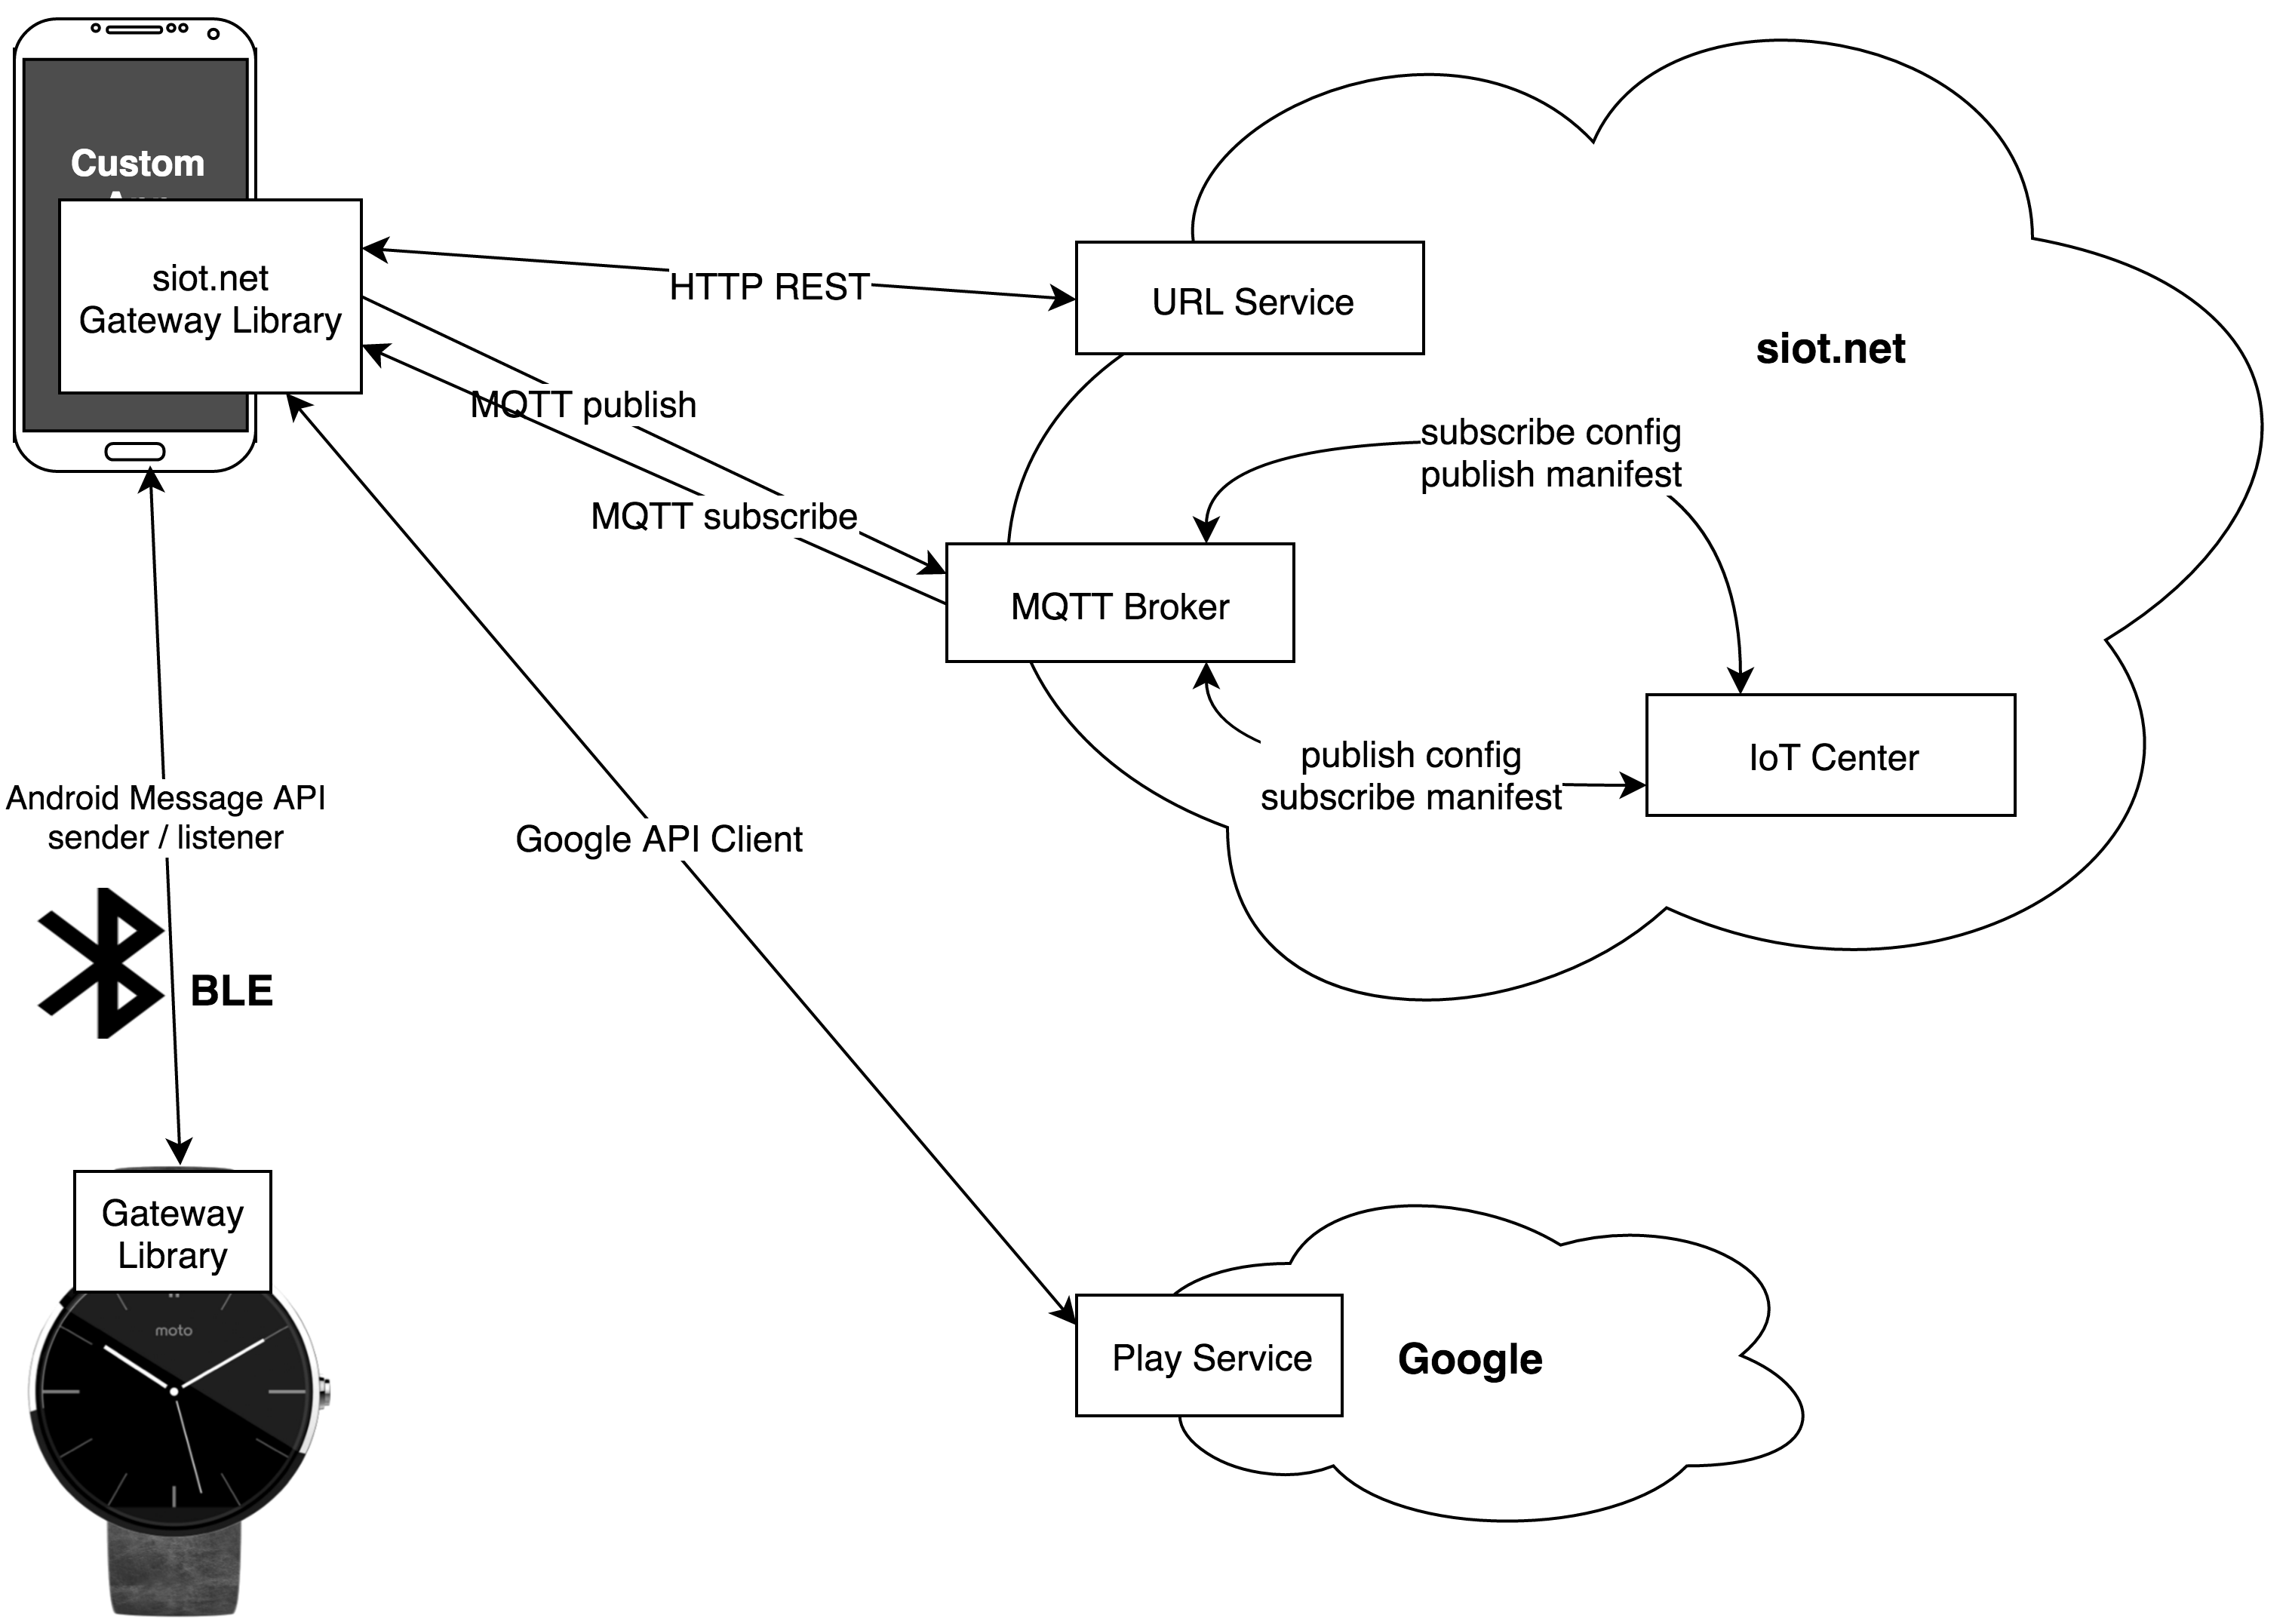
\includegraphics[scale=0.15]{98_Bilder/07_Architektur/03_Architektur}
  \caption[Effektive Netzwerk-Architektur mit BLE/ohne WLAN]{Effektive Kommunikation zwischen Smartwatch und siot.net, sowie Smartphone und siot.net}
\end{figure}
Diese Architektur (siehe Abbildung 7.5) unterscheidet sich geringfügig zu jener Abbildung 7.3. Hier kommt nun die Google Cloud dazu. Dies ist notwendig, da Android nicht erlaubt direkt über die Android Message API zu kommunizieren. Es muss vorhergehend eine NodeId über den Google Play Service eingefordert werden. Dank dieser NodeId dürfen die Geräte (Smartphone und Smartwatch benötigen eine eindeutige Identifikation) mittels Message API Nachrichten transferieren. Der Datenaustausch geschieht dann direkt via BLE. Dies ist die Netzwerk-Architektur kommt zum tragen, wenn die Kopplung von Smartwatch und Smartphone über Bluetooth Smart steht.

\newpage
\begin{figure}[h]
  \centering
  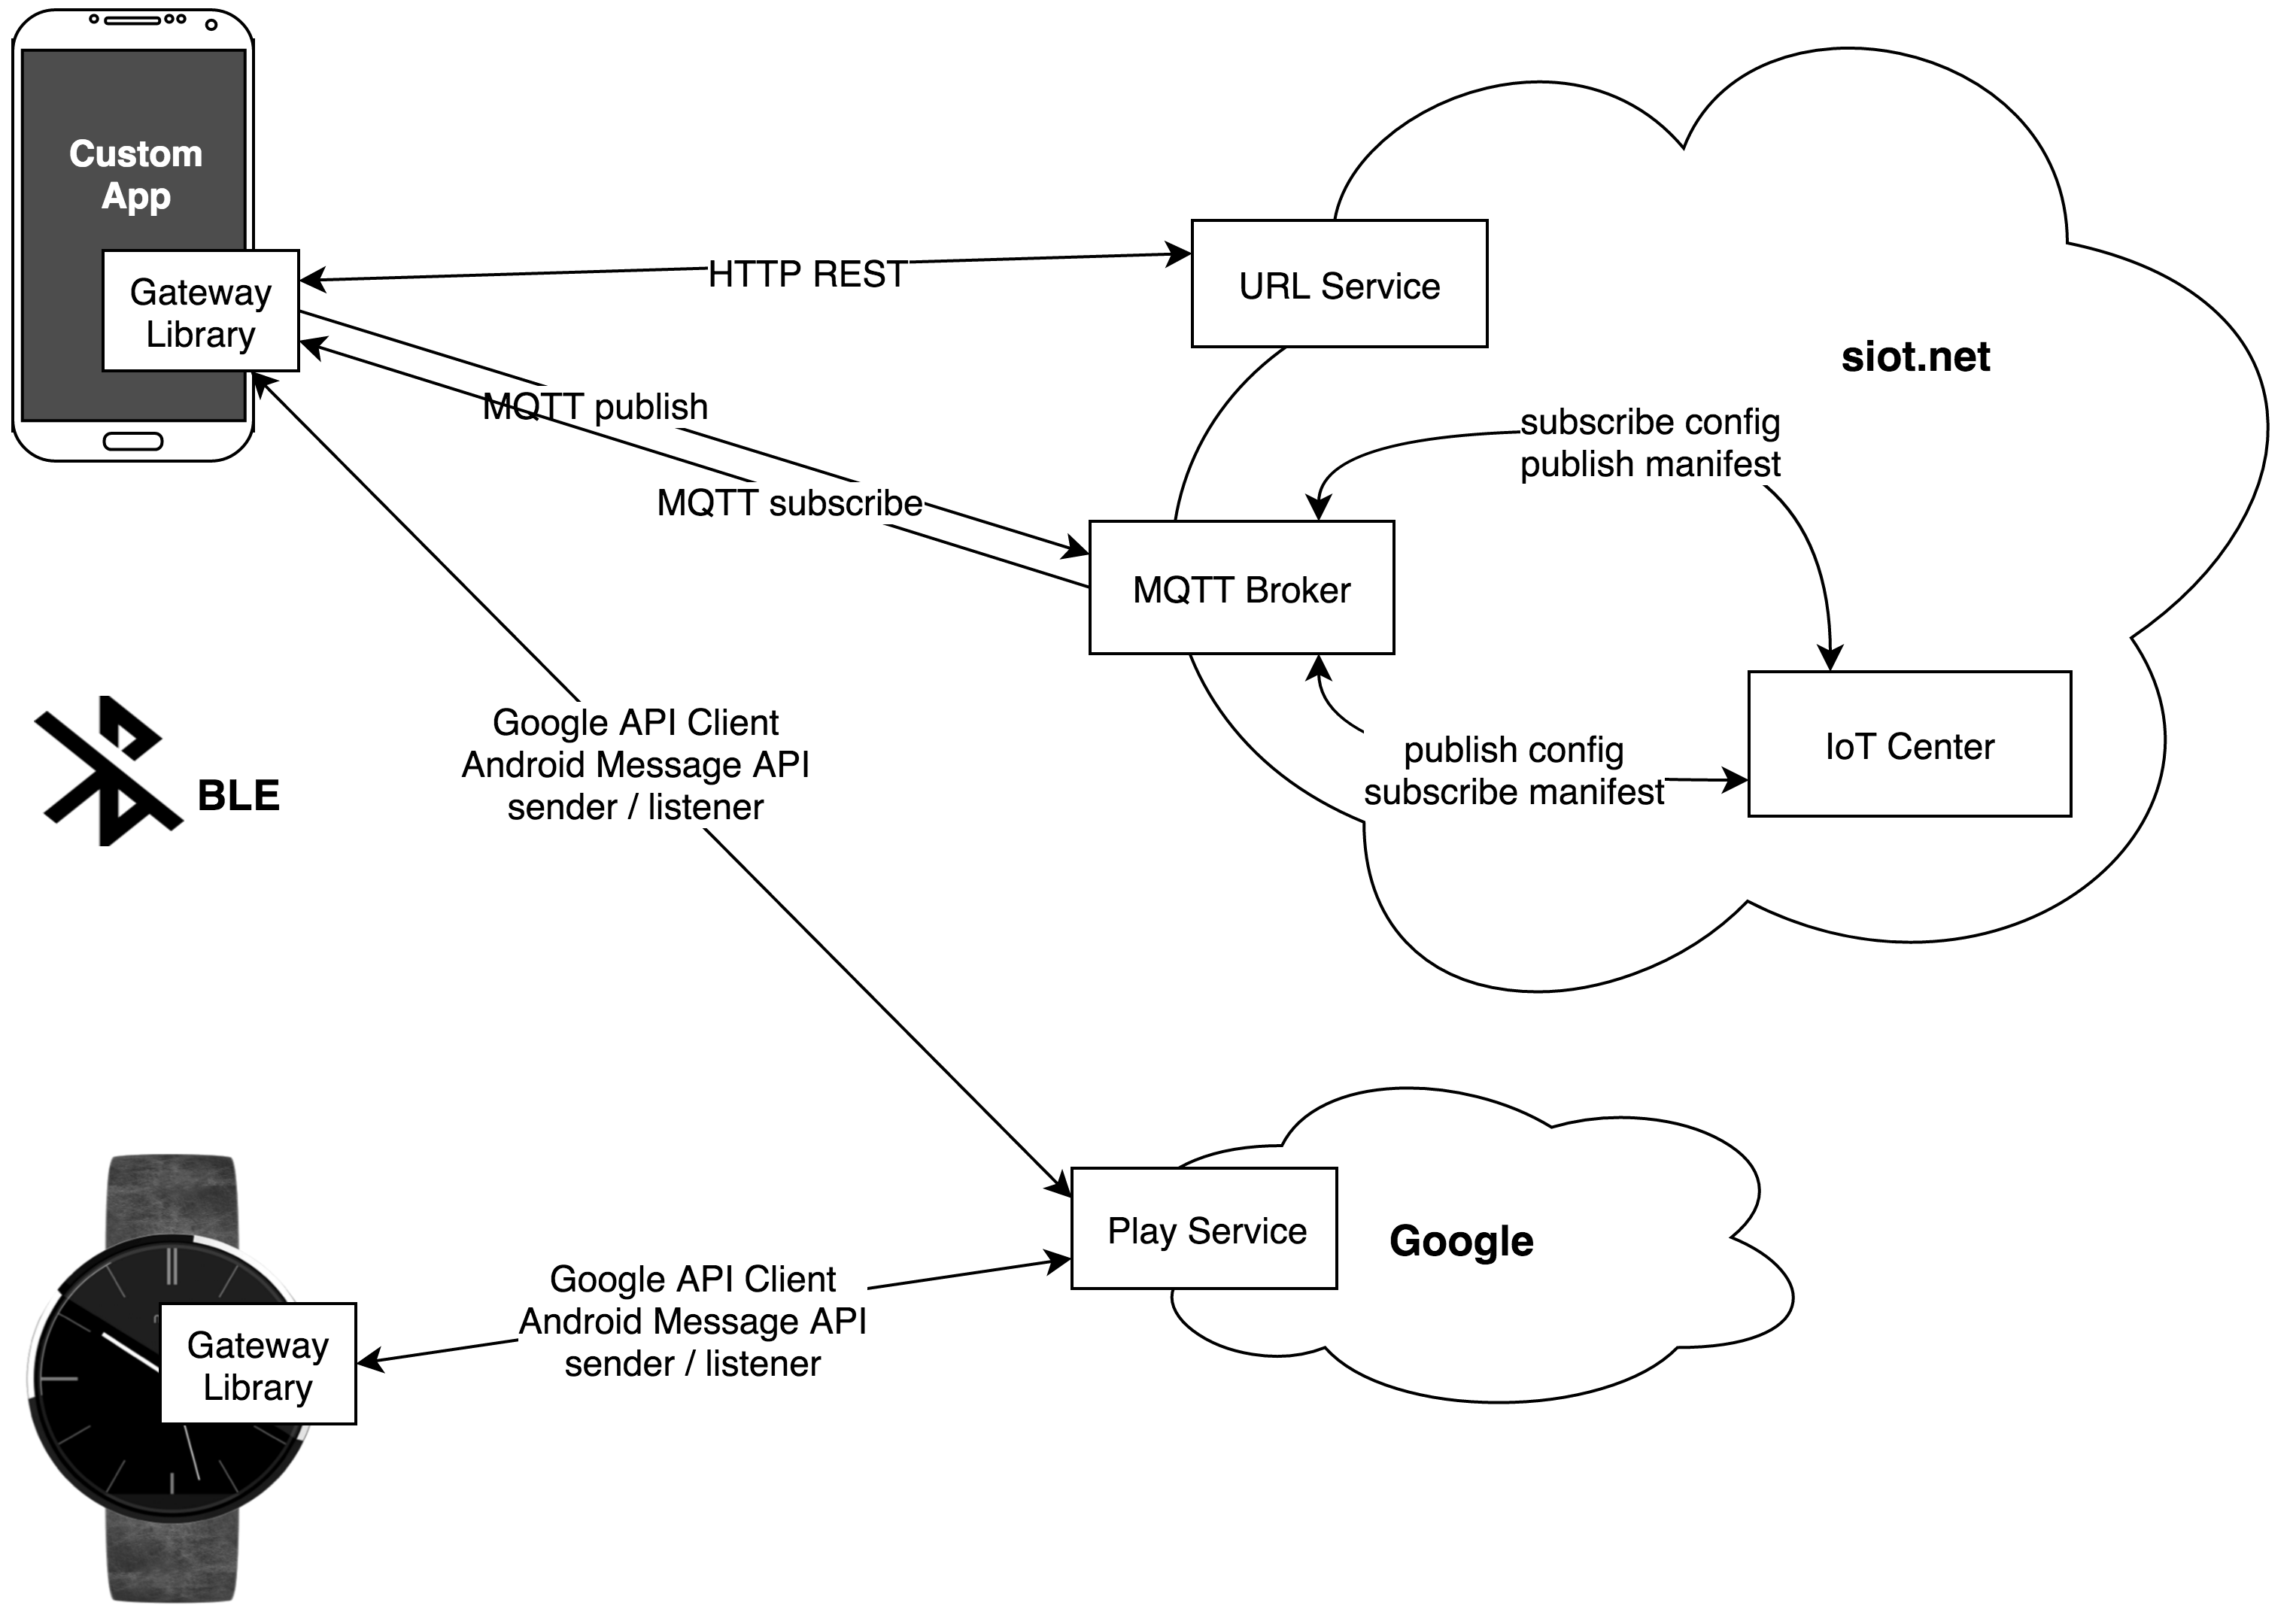
\includegraphics[scale=0.15]{98_Bilder/07_Architektur/04_Architektur}
  \caption[Effektive Netzwerk-Architektur mit BLE/ohne WLAN]{Effektive Kommunikation zwischen Smartwatch und siot.net, sowie Smartphone und siot.net}
\end{figure}
Abbildung 7.6 zeigt die funktionierende Architektur. Diese differenziert sich wesentlich von der geplanten Netzwerk-Definition. Auch hier spielt der Faktor Android eine grosse Rolle, denn es verbietet Android Wear Geräten den direkten Kontakt zum Internet. So ist hier eine Verbindung über den Google Play Service zum Smartphone nötig. Bei dieser Anbindungsart werden die Daten via Google Cloud an das Android Handy gesendet. Es muss in jedemfall die Verbindung zu siot.net verwalten.\\
Der grosse Nachteil dieser Variante ist, dass die Smartwatch nicht als autonomes Gerät fungieren kann. Wenn das Smartphone nicht erreichbar ist, z.B. Akku leer, keine Netzverbindung, ist die Smartwatch für siot.net nutzlos.
